\documentclass[conference]{IEEEtran}
\IEEEoverridecommandlockouts
% The preceding line is only needed to identify funding in the first footnote. If that is unneeded, please comment it out.
\usepackage[utf8]{inputenc}
\usepackage[greek,english]{babel}
\usepackage{alphabeta}
\usepackage{cite}
\usepackage{amsmath,amssymb,amsfonts}
\usepackage{algorithmic}
\usepackage{graphicx}
\usepackage{textcomp}
\usepackage{xcolor}
\usepackage{pgfplots}
\pgfplotsset{compat=1.16}

\def\BibTeX{{\rm B\kern-.05em{\sc i\kern-.025em b}\kern-.08em
    T\kern-.1667em\lower.7ex\hbox{E}\kern-.125emX}}
\begin{document}

\title{Key-Value stores Riak vs ArangoDB \\

}

\author{\IEEEauthorblockN{Αγγελου Στελιος}
\IEEEauthorblockA{
% \textit{National Technical University of Athens} \\
% \textit{Electrical and Computer Egineering}\\
αριθμος μητρώου
}
\and
\IEEEauthorblockN{Γκέργκες Μάρκος}
\IEEEauthorblockA{
03117870 
}
\and
\IEEEauthorblockN{Παπαβασιλόπουλος Παναγιώτης-Φίλιππος}
\IEEEauthorblockA{
03117444
}
}

\maketitle

\begin{abstract}
    Τα τελευταία χρόνια η ανάπτυξη των συστημάτων 
διαχείρισης βάσεων δεδομένων (DBMS) είναι αναπόφευκτη προκειμένου να 
ανταποκριθούμε στη ραγδαία αύξηση των δεδομένων που 
αποθηκεύονται. Στην προσπάθεια διαχείρισης big data 
πολλές φορές μπορεί να κληθεί να επιλέξει κανείς την 
βάση δεδομένων που θα ανταποκριθεί καλύτερα στον σκοπό 
που επιδιώκει. Επικουρικό σκοπό σε αυτό έχουν benchmarking 
tools όπως το Yahoo! Cloud Service Benchmark.

\end{abstract}

\begin{IEEEkeywords}
component, formatting, style, styling, insert
\end{IEEEkeywords}

\section{Introduction}

\section{Σκοπός της εργασίας}

Σε αυτή την εργασία θα γίνει σύγκριση όσο αφορά την φόρτωση δεδομένων, select queries, range queries,
update queries, delete queries, insert queries, των δύο key-value stores Riak και ArangoDB. Θα γίνει
σύγκριση των δύο key-value stores σε διάφορες περιπτώσεις όπως αναφέρεται παρακάτω. Στην συγκεκριμένη εργασία θα
χρησιμοποιηθεί το γνωστό tool YCSB benchmark.
% Σε αυτή την εργασία θα γίνει σύγκριση όσον αφορά την φόρτωση δεδομένων, select queries, range queries, update queries και κλιμακωσιμότητα σε μεγάλου όγκου δεδομένα ανάμεσα σε δύο από τις γνωστές NoSQL databases: Riak, Arangodb. Θα χρησιμοποιηθεί το γνωστό YCSB benchmark.


\section{Περιγραφή βημάτων για το στήσιμο του συστήματος και των πειραμάτων}
Before you begin to format your paper, first write and save the content as a 
separate text file. Complete all content and organizational editing before 
formatting. Please note sections \ref{AA}--\ref{SCM} below for more information on 
proofreading, spelling and grammar.

Keep your text and graphic files separate until after the text has been 
formatted and styled. Do not number text heads---{\LaTeX} will do that 
for you.

\section{Περιγραφή της υποδομής και του software που χρησιμοποίηθηκε}

\subsection{Okeanos}
Για να κάνουμε τις μετρήσεις που χρησιμοποιήθηκαν στην εργασία χρησιμοποιήσαμε το cloud service okeanos-knossos που παρέχει το Εθνικό Δίκτυο Υποδομών Τεχνολογίας και Έρευνας (GRNET). Mε τους πόρους που μας δόθηκαν στήσαμε 3 Virtual Machines με τα εξής χαρακτηριστικά:
\begin{itemize}

\item
1ο VM: 4CPU’s 8GB RAM όπου περιέχει το YCSB
\item
2ο VM: 2CPU’s 4GB RAM όπου τρέχουμε την Arangodb
\item
3ο VM: 2CPU’s 4GB RAM όπου τρέχουμε την Riak  που έπειτα το αναβαθμίσαμε σε 4CPU’s 8GB RAM

\end{itemize}

\subsection{Yahoo Cloud Service Benchmark}
        To Yahoo! Cloud Serving Benchmark (YCSB) είναι μία open-source συλλογή προγραμμάτων που βοηθάει στην αξιολόγηση τον δυνατοτήτων άλλων προγραμμάτων όπως την απόδοση NoSQL συστημάτων διαχείρισης βάσεων δεδομένων (DBMS). Δημιουργήθηκε από το ερευνητικό τμήμα της Yahoo! με πρώτη έκδοση το 2010 και έκτοτε έχει χρησιμοποιηθεί πολύ συχνά από τους παρόχους DBMS για την σύγκριση του προϊόντος τους με των ανταγωνιστών (benchmark marketing) και για ακαδημαϊκούς, ερευνητικούς και διδακτικούς σκοπούς. Μπορεί να συγκρίνει πολλές βάσεις δεδομένων με διαφορετική αρχιτεκτονική μετρώντας τον τρόπο που ανταποκρίνονται σε ποικίλου είδους εργασιών (workloads) περισσότερες λεπτομέρειες για τα οποία θα αναφέρουμε σε επόμενες παραγράφους.
       
        Το YCSB εστιάζει σε συστήματα που παρέχουν online read/write access σε data. Παραδείγματα είναι ένας χρήστης να αναμένει μία ιστοσελίδα να χορτώσει (load) και έπειτα να διαβάζει και να γράφει δεδομένα που αποθηκεύονται σε μία βάση. Από την άλλη μεριά συστήματα όπως το Hadoop ή  άλλα relational OLAP συστήματα κυρίως εστιάζουν σε offline και near-line queries.
	   
        To framework του YCSB αποτελείται από έναν client-δημιουργό workloads και από έτοιμα workloads τα οποία καλύπτουν μεγάλο εύρος των ελέγχων απόδοσης των DBMS. Σημαντικό χαρακτηριστικό λοιπόν είναι η επεκτασιμότητα του YCSB καθώς είναι ιδιαίτερα εύκολη η δημιουργία workloads με τα οποία απαιτεί ο χρήστης να κάνει την σύγκριση με τις δικές του απαιτήσεις. Το YCSB είναι open-source για να μπορούν οι developers να κάνουν πειράματα εύκολα και να συνεισφέρουν με τα workloads που δημιούργησαν προκειμένου να γίνονται διαρκώς νέες ενδιαφέρουσες παρατηρήσεις.

        Κάθε σύστημα έκανε διαφορετικές αρχιτεκτονικές επιλογές για την διεξαγωγή των queries καθώς κανένα σύστημα δεν είναι ιδανικό για όλα τα workloads. Διαφορετικά συστήματα κάνουν άλλους συμβιβασμούς κατα την διεξαγωγή διαφόρου τύπου εφαρμογών. Τέτοιοι συμβιβασμοί περιλαμβάνουν: 
        \begin{itemize}
        \item
        Έμφαση στην απόδοση σε Reads από Write εντολές και αντίστροφα καθώς είναι δύσκολη η πρόβλεψη ποιο record θα γίνει read ή written.
        \item
        Επιλογή ανάμεσα σε χαμηλή καθυστέρηση (latency) έναντι ανθεκτικότητας (durability) λόγω της μεταφοράς των δεδομένων από και προς τον δίσκο καθώς μπορεί να αποφύγουν να γραφτούν κάποια δεδομένα που επεξεργάζονται στον δίσκο γεγονός που ανεβάζει την ταχύτητα αλλά σε περίπτωση crash τα αποτελέσματα θα είναι δυσάρεστα.
        \item
        Την σύγχρονη έναντι της ασύγχρονης αντιγραφής των δεδομένων των συστημάτων με την αντιγραφή των δεδομένων σε πολλά διαφορετικά αντίγραφα για τον περιορισμό της απώλειας δεδομένων
        \item
        Τον διαχωρισμό των δεδομένων του συστήματος σε γραμμές ή στήλες ανάλογα αν είναι επιθυμητή ή πρόσβαση γρήγορα σε λίγα records είτε η πρόσβαση σε υποσύνολα στηλών πολλαπλών records.
    \end{itemize}

Τέτοιου είδους συμβιβασμοί εκτιμούμε ότι θα οδηγήσουν σε διαφορετικά αποτελέσματα ανάμεσα στην ArangoDB και τη Riak όταν τις μελετήσουμε και τις συγκρίνουμε στη συνέχεια με τη χρήση του εργαλείου YCSB.

\subsection{ArangoDB}
Η ArangoDB είναι μια ανοιχτού κώδικά βάση δεδομένων NoSQL. Χαρακτηριστικό της είναι ο ευέλικτος τρόπος μοντελοποίσης των δεδομένων σε documents ή γράφους. Έχει σχεδιαστεί ως «βάση δεδομένων γενικού σκοπού», προσφέροντας όλες τις λειτουργίες που απαιτούνται συνήθως για τις σύγχρονες εφαρμογές Ιστού. Υποστηρίζει μοντέλα δεδομένων γραφημάτων, εγγράφων και κλειδιών-τιμών που επιτρέπουν στους χρήστες να συνδυάζουν ελεύθερα όλα τα μοντέλα δεδομένων σε ένα μόνο query. Καθώς οι εφαρμογές γίνονται όλο και πιο περίπλοκες, συχνά χρειαζόμαστε περισσότερες από μία βάσεις δεδομένων NoSQL. Η χρήση μιας βάσης δεδομένων πολλαπλών μοντέλων μπορεί να απλοποιήσει την αρχιτεκτονική μας συνδυάζοντας πολλούς τύπους NoSQL σε μια ενιαία υποδομή.

Σύμφωνα με αυτό, θα μπορούσε κανείς, για παράδειγμα, να χρησιμοποιήσει μια σχεσιακή βάση δεδομένων για να διατηρήσει δομημένα, πινακοποιημένα δεδομένα. ένα χώρο αποθήκευσης εγγράφων για μη δομημένα δεδομένα που μοιάζουν με αντικείμενα. ένα κατάστημα κλειδιού/τιμής για έναν πίνακα κατακερματισμού. και μια βάση δεδομένων γραφημάτων για ιδιαίτερα συνδεδεμένα αναφορικά δεδομένα.

Ωστόσο, η παραδοσιακή εφαρμογή αυτής της προσέγγισης θα οδηγήσει κάποιον στη χρήση πολλαπλών βάσεων δεδομένων στο ίδιο project. Μπορεί να οδηγήσει σε κάποιες λειτουργικές τριβές (πιο περίπλοκη ανάπτυξη, πιο συχνές αναβαθμίσεις) καθώς και σε ζητήμα τα συνέπειας και συντήρησης των ίδων δεδομένων πολλαπλές φορές.

Ποια ειναι τα κύρια χαρακτηριστικά της ArangoDB;
\begin{itemize}
    \item 
    Δυνατότητα για χρησιμοποίηση διαφορετικών τεχνολογιών αποθήκευσης, που ταιριάζουν καλύτερα με τον τρόπο που χρησιμοποιούνται τα δεδομένα από διαφορετικά στοιχεία της εφαρμογής.
    
    \item 
    Προσφέρεται πρόσβαση σε οποιαδήποτε δεδομένα (ανεξάρτητα από το μοντέλο τους) χρησιμοποιώντας μια ενιαία γλώσσα ερωτημάτων, η οποία είναι αρκετά παρόμοια με μια τυπική γλώσσα ερωτήματος SQL με κάποιες μικρές διαφορές.

    \item 
    Χρησιμοποιεί δυαδικό JSON για την αποθήκευση δεδομένων. Είναι λιτό, αυτόνομο, βελτιώνει τις απαιτήσεις από μνήμη και καλύπτει όλους τους JSON τύπους δεδομένων συν ημερομηνίες, δυαδικά δεδομένα, ακέραιους αριθμούς, καθώς και αυθαίρετους αριθμούς ακριβείας.
\end{itemize}

ArangoDB: A distributed open-source database with a flexible data model for documents, graphs, and key-values. A distributed free and open-source database with a flexible data model for documents, graphs, and key-values. Build high performance applications using a convenient SQL-like query language or JavaScript extensions;

\subsection{Riak KV}

 Η Riak είναι μια κατανεμημένη βάση δεδομένων που έχει σχεδιαστεί για να παρέχει τη μέγιστη διαθεσιμότητα δεδομένων, διανέμοντας τα δεδομένα σε πολλούς διακομιστές. Εφόσον ο client μπορεί να φτάσει σε έναν διακομιστή Riak, θα πρέπει να μπορεί να γράψει δεδομένα.

H Riak χρησιμοποιείται ως ένα eventually consistent σύστημα, καθώς τα δεδομένα σε read operations θα πρέπει να παραμένουν διαθέσιμα στα περισσότερα σενάρια αποτυχίας, αν και μπορεί να μην είναι η πιο ενημερωμένη έκδοση αυτών των δεδομένων τη δεδομένη στιγμή, λόγω του eventual consistency.

Ποια ειναι τα κύρια χαρακτηριστικά της Riak KV;
\begin{itemize}
    \item 
    Διαθεσιμότητα - H Riak γράφει και διαβάζει από πολλούς διακομιστές για να προσφέρει διαθεσιμότητα δεδομένων ακόμα και όταν το υλικό ή το ίδιο το δίκτυο αντιμετωπίζει συνθήκες αποτυχίας.(π.χ. network partitioning, node failure, κλπ.)
    
    \item 
    Επεκτασιμότητα - Η Riak διανέμει αυτόματα τα δεδομένα στο cluster και αποφέρει σχεδόν γραμμική αύξηση απόδοσης καθώς προστίθενται κόμβοι στο cluster.

    \item 
    Τα αιτήματά δεν είναι όμηρα ενός συγκεκριμένου διακομιστή στο cluster που μπορεί να είναι ή να μην είναι διαθέσιμο, αφού δεν υπάρχει master κόμβος. Η Riak επιτρέπει την ανάγνωση και την εγγραφή σε οποιοδήποτε διαθέσιμο κόμβο στο cluster.
\end{itemize}
Το απλό μοντέλο δεδομένων της Riak, που αποτελείται από κλειδιά και τιμές ως ατομικά του στοιχεία, σημαίνει ότι τα δεδομένα πρέπει να ειναι denormalized για να είναι το σύστημά εύλογα αποδοτικό. Αντίστοιχα, εάν η εφαρμογή απαιτεί υψηλό φορτίο ερωτημάτων με range εκτός από την αναζήτηση κλειδιού/τιμής - λειτουργίες τύπου SQL — h Riak δεν θα είναι τόσο αποτελεσματική όσο άλλες βάσεις δεδομένων.



\subsection{Docker}


\section{Περιγραφή των αποτελεσμάτων και των συμπερασμάτων της εργασίας}

Χρησιμοποιήθηκαν workloads από το core package του ycsb. Αυτά έχουν οριστεί ανάλογα με τι εντολές θα εκτελεστούν και με σε τι ποσοστό η κάθε μία αλλά και με ποιόν τρόπο θα γίνεται η επιλογή ποιο record θα γίνει read και ποιο write. Τα Workloads Α και B που βάλαμε στα DBMS επιλέγουν τα records σύμφωνα με την Zipfian κατανομή και περιλαμβάνουν λειτουργίες:
\begin{itemize}
\item 
Workload A: 50/100 Read - 50/100 Update
\item 
Workload A: 95/100 Read - 5/100 Update (Heavy Read)
\end{itemize}


\subsection{Workload A}    

Αρχικά εξετάζουμε πως ανταποκρίνονται οι ArangoDB και Riad στο Workload A το οποίο περιλαμβάνει 50/100 Reads, 50/100 Updates.  Μία εφαρμογή τέτοιου workload αποτελούν τα session stores πχ. Cookies ενός browser.  Στα διαγράμματα παρουσιάζεται η καθυστέρηση (latency) συναρτήσει του throughput αρχικά για τα Reads και έπειτα για τα  Updates του Workload A. Σε κάθε περίπτωση αυξάναμε το δυνατό throughput μέχρις ότου παρατηρούσαμε ότι σταματούσε να αυξάνεται. Παρατηρούμε ότι σε όλα τα συστήματα, όσο αυξάνουμε το δυνατό throughput τόσο ανεβαίνει και το latency. Το καλύτερο throughput το πέτυχε η ArangoDB και το μικρότερο latency και στην περίπτωση των Reads και στην περίπτωση των updates. 


This workload has a mix of 50/50 reads and writes. An application example is a session store 
recording recent actions. Updates in this workload do not presume you read the original record first. 
The assumption is all update writes contain fields for a record that already exists; oftentimes writing 
only a subset of the total fields for that record. Some data stores need to read the underlying record 
in order to reconcile what the final record should look like, but not all do.

% Fist diagram Workload a - run operations
    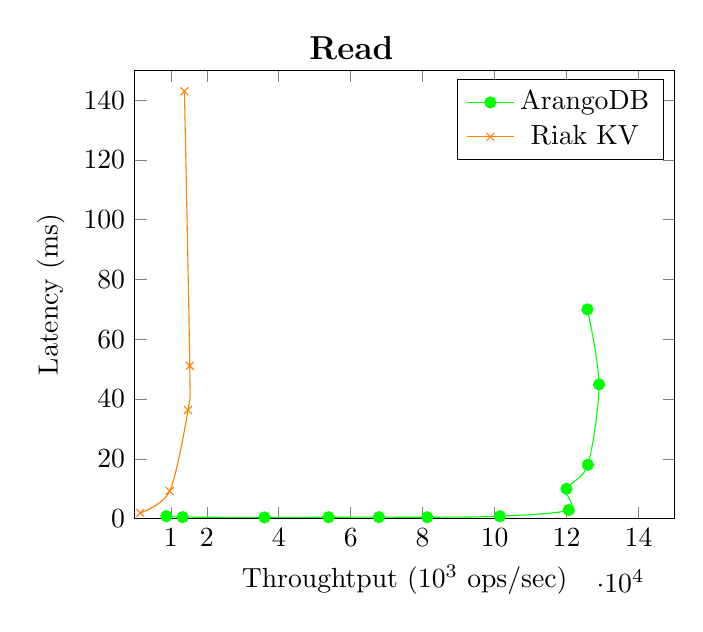
\begin{tikzpicture}
\begin{axis}[
    xlabel=Throughtput ($10^{3}$ ops/sec),
    ylabel=Latency (ms),
    xmin=0, xmax=15000,
    ymin=0, ymax=150,
    xtick={1000, 2000,4000, 6000, 8000,10000,12000, 14000},
    xticklabels={1, 2, 4, 6, 8, 10, 12, 14},
    ytick={0,20,...,160}
            ]
\addplot[smooth,color=green,mark=*] plot coordinates {
    (876,0.8)
    (1329,0.5)
    (3603,0.4)
    (5385,0.45)
    (6782,0.49)
    (8127,0.45)
    (10145,0.8)
    (12062, 2.9)
    (11995, 9.961)
    (12592, 18)
    (12903, 44.884)
    (12581, 70)
};
\addlegendentry{ArangoDB}

\addplot[smooth,color=orange,mark=x]
    plot coordinates {
    (149,1.9)
    (969,9.219)
    (1476,36.330)
    (1526,51.128)
    (1378,142.990)
    };
\addlegendentry{Riak KV}
\end{axis}
\node[above,font=\large\bfseries] at (current bounding box.north) {Read};

    \end{tikzpicture}


% Second diagram Workload a - write operations
    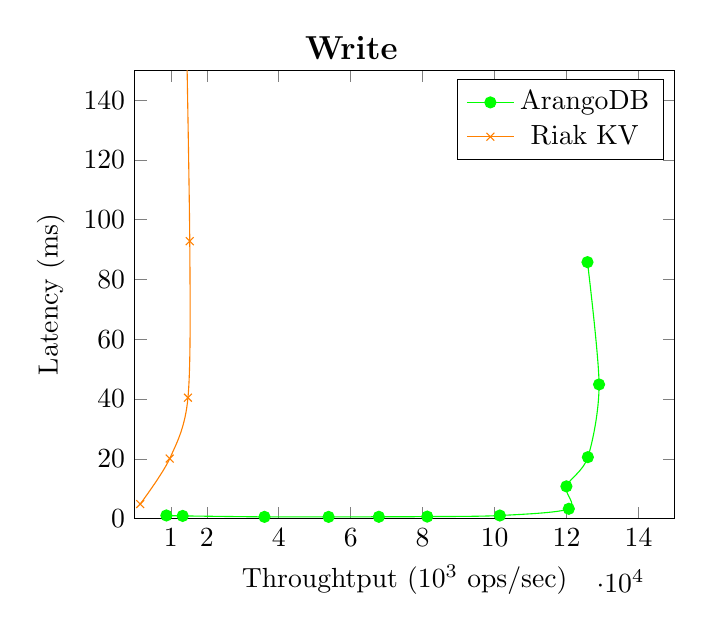
\begin{tikzpicture}
\begin{axis}[
    xlabel=Throughtput ($10^{3}$ ops/sec),
    ylabel=Latency (ms),
    xmin=0, xmax=15000,
    ymin=0, ymax=150,
    xtick={1000, 2000,4000, 6000, 8000,10000,12000, 14000},
    xticklabels={1, 2, 4, 6, 8, 10, 12, 14},
    ytick={0,20,...,160}
            ]
\addplot[smooth,color=green,mark=*] plot coordinates {
    (876,1.046)
    (1329,0.902)
    (3603,0.582)
    (5385, 0.577)
    (6782, 0.609)
    (8127, 0.670)
    (10145, 1.031)
    (12062, 3.279)
    (11995,  10.787)
    (12592, 20.565)
    (12903, 44.884)
    (12581, 85.810)
};
\addlegendentry{ArangoDB}

\addplot[smooth,color=orange,mark=x]
    plot coordinates {
        (149, 4.867)
        (969, 20.091)
        (1476, 40.452)
        (1526,92.816)
        (1378,198.836)
    };
\addlegendentry{Riak KV}
\end{axis}

\node[above,font=\large\bfseries] at (current bounding box.north) {Write};
    \end{tikzpicture}

    
\subsection{Workload b}
    To Workload B είναι heavy Read (95/100 Read - 5/100 Updates) και μία εφαρμογή του είναι η προσθήκη ετικετών σε φωτογραφίες (photo tagging) όπου η προσθήκη tag είναι ένα Update όμως κυρίως είναι η ανάγνωση ετικετών. Πάλι η ArangoDB είχε μεγαλύτερο throughput και μικρότερο latency. To μέγιστο throughput της ArangoDB ήταν λίγο καλύτερο στην περίπτωση του Workload A από το Workload B.

%Third Diagram Workload b
%  Read s
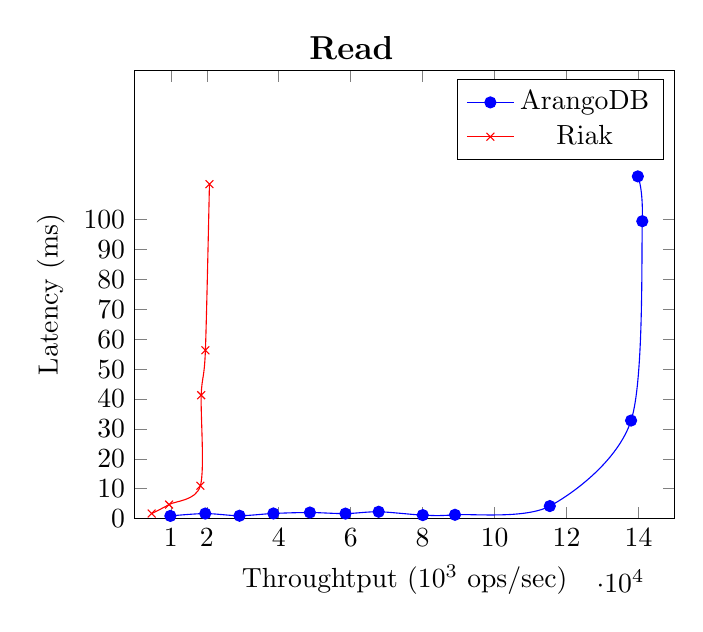
\begin{tikzpicture}
    \begin{axis}[
        xlabel=Throughtput ($10^{3}$ ops/sec),
        ylabel=Latency (ms),
        xmin=0, xmax=15000,
        ymin=0, ymax=150,
        xtick={1000, 2000,4000, 6000, 8000,10000,12000, 14000},
        xticklabels={1, 2, 4, 6, 8, 10, 12, 14},
        ytick={0,10,...,100}
                ]
    \addplot[smooth,mark=*,blue] plot coordinates {
        (987,0.9)
        (1957,1.69)
        (2909,0.96)
        (3850,1.72)
        (4866,2.04)
        (5854,1.67)
        (6777,2.29)
        (8003, 1.17)
        (8898, 1.27)
        (11534, 4.19)
        (13793, 32.810)
        (14105, 99.5)
        (13981,114.5)
    };
    \addlegendentry{ArangoDB}
    
    \addplot[smooth,color=red,mark=x]
        plot coordinates {
            (466.8,1.69)
            (950.9,4.7)
            (1821,10.98)
            (1844,41.29)
           (1961,56.31)
           (2073,111.9)
            
        };
    \addlegendentry{Riak}
    \end{axis}
    \node[above,font=\large\bfseries] at (current bounding box.north) {Read};
    
        \end{tikzpicture}

%Fourth Diagram Workload b Update
%  Read s
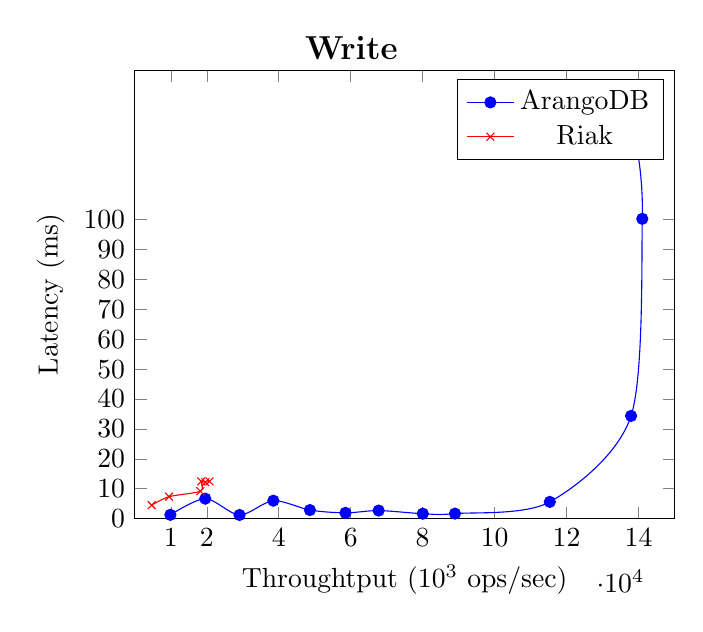
\begin{tikzpicture}
    \begin{axis}[
        xlabel=Throughtput ($10^{3}$ ops/sec),
        ylabel=Latency (ms),
        xmin=0, xmax=15000,
        ymin=0, ymax=150,
        xtick={1000, 2000,4000, 6000, 8000,10000,12000, 14000},
        xticklabels={1, 2, 4, 6, 8, 10, 12, 14},
        ytick={0,10,...,100}
                ]
    \addplot[smooth,mark=*,blue] plot coordinates {
        (987,1.26)
        (1957,6.66)
        (2909,1.214)
        (3850,5.99)
        (4866,2.86)
        (5854,1.92)
        (6777,2.69)
        (8003, 1.64)
        (8898, 1.669)
        (11534, 5.596)
        (13793, 34.36)
        (14105, 100.3)
        (13981,122.1)
    };
    \addlegendentry{ArangoDB}
    
    \addplot[smooth,color=red,mark=x]
        plot coordinates {
            (466.8,4.49)
            (950.9,7.33)
            (1821,9.17)
            (1844,12.46)
           (1961,12.17)
           (2073,12.45)
            
        };
    \addlegendentry{Riak}
    \end{axis}
    \node[above,font=\large\bfseries] at (current bounding box.north) {Write};
    
        \end{tikzpicture}

\subsection{Διπλασιάζοντας του πόρους της Riak}

\subsubsection{Workload a - Updates}
Από το worklfow a θα συγκρίνουμε τις επιδόσεις στα reads, μιας και τα reads θα εξετασθούν από το heavy-read workflow b.

%Fifth Diagram Workload a Update
%  Writes
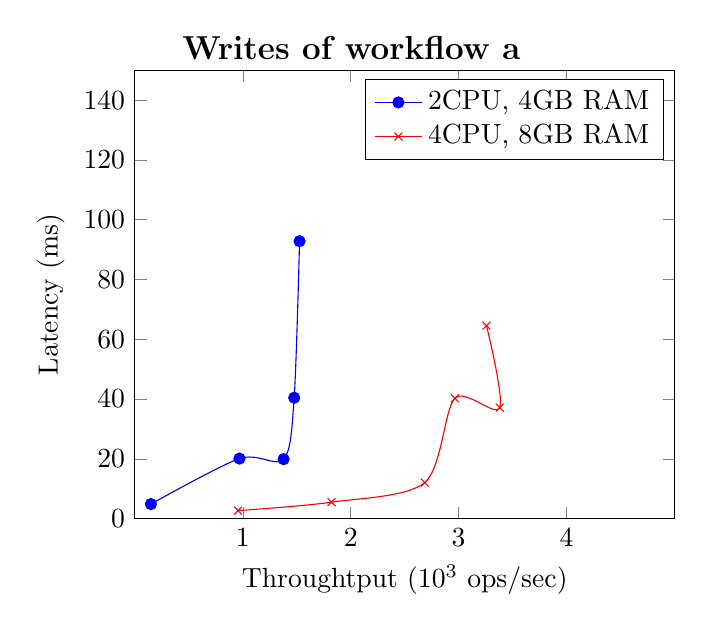
\begin{tikzpicture}
    \begin{axis}[
        xlabel=Throughtput ($10^{3}$ ops/sec),
        ylabel=Latency (ms),
        xmin=0, xmax=5000,
        ymin=0, ymax=150,
        xtick={1000,2000,3000, 4000},
        xticklabels={1,2,3, 4},   % <---
        ytick={0,20,...,150}
                ]
    \addplot[smooth,mark=*,blue] plot coordinates {
        (149, 4.867)
        (969, 20.091)
        (1378,19.8836)
        (1476, 40.452)
        (1526,92.816)

    };
    \addlegendentry{2CPU, 4GB RAM}
    
    \addplot[smooth,color=red,mark=x]
        plot coordinates {
            (956, 2.686)
            (1822, 5.497)
            (2686, 12.037)
            (2965, 40.240)
            (3381, 37.114)
            (3258, 64.592)
        };
    \addlegendentry{4CPU, 8GB RAM}
    \end{axis}
    \node[above,font=\large\bfseries] at (current bounding box.north) {Writes of workflow a};
    
        \end{tikzpicture}


\subsubsection{Workload b - Reads}
%Sixth Diagram Workload b Reads
%  Read s
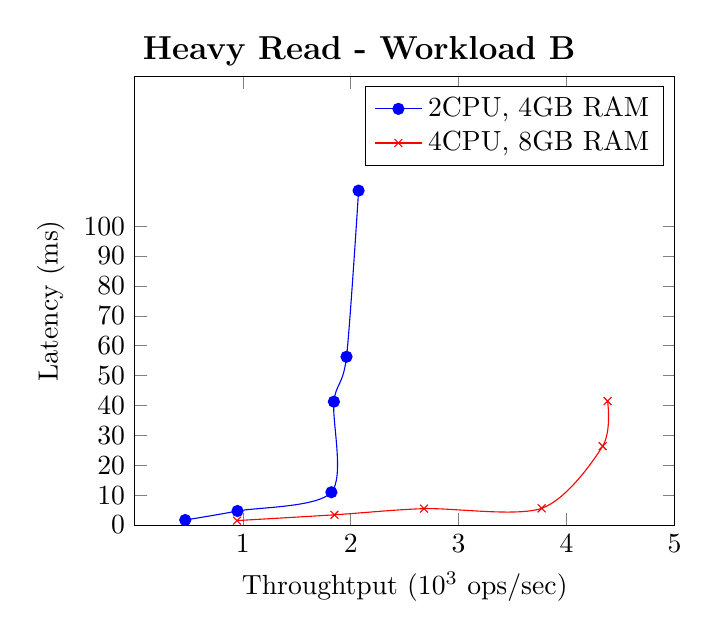
\begin{tikzpicture}
    \begin{axis}[
        xlabel=Throughtput ($10^{3}$ ops/sec),
        ylabel=Latency (ms),
        xmin=0, xmax=5000,
        ymin=0, ymax=150,
        xtick={1000, 2000, 3000, 4000, 5000},
        xticklabels={1,2, 3, 4, 5 },   % <---
        ytick={0,10,...,100}
                ]
    \addplot[smooth,mark=*,blue] plot coordinates {
        (466.8,1.69)
        (950.9,4.7)
        (1821,10.98)
        (1844,41.29)
        (1961,56.31)
        (2073,111.9)


    };
    \addlegendentry{2CPU, 4GB RAM}
    
    \addplot[smooth,color=red,mark=x]
        plot coordinates {
            (946.7,1.5)
            (1849,3.43)
            (2679,5.49)
            (3769,5.6)
            (4334,26.4)
            (4380,41.48)
            
        };
    \addlegendentry{4CPU, 8GB RAM}
    \end{axis}
    \node[above,font=\large\bfseries] at (current bounding box.north) {Heavy Read - Workload B};
    
        \end{tikzpicture}


\section{βιβλιογραφία και παραπομπές που χρησιμοποιήθηκαν στο κείμενο}

\subsection{Abbreviations and Acronyms}\label{AA}
Define abbreviations and acronyms the first time they are used in the text, 
even after they have been defined in the abstract. Abbreviations such as 
IEEE, SI, MKS, CGS, ac, dc, and rms do not have to be defined. Do not use 
abbreviations in the title or heads unless they are unavoidable.

\subsection{abcd}
\begin{itemize}
\item Use either SI (MKS) or CGS as primary units. (SI units are encouraged.) English units may be used as secondary units (in parentheses). An exception would be the use of English units as identifiers in trade, such as ``3.5-inch disk drive''.
\item Avoid combining SI and CGS units, such as current in amperes and magnetic field in oersteds. This often leads to confusion because equations do not balance dimensionally. If you must use mixed units, clearly state the units for each quantity that you use in an equation.
\item Do not mix complete spellings and abbreviations of units: ``Wb/m\textsuperscript{2}'' or ``webers per square meter'', not ``webers/m\textsuperscript{2}''. Spell out units when they appear in text: ``. . . a few henries'', not ``. . . a few H''.
\item Use a zero before decimal points: ``0.25'', not ``.25''. Use ``cm\textsuperscript{3}'', not ``cc''.)
\end{itemize}

\subsection{Equations}
Number equations consecutively. To make your 
equations more compact, you may use the solidus (~/~), the exp function, or 
appropriate exponents. Italicize Roman symbols for quantities and variables, 
but not Greek symbols. Use a long dash rather than a hyphen for a minus 
sign. Punctuate equations with commas or periods when they are part of a 
sentence, as in:
\begin{equation}
a+b=\gamma\label{eq}
\end{equation}

Be sure that the 
symbols in your equation have been defined before or immediately following 
the equation. Use ``\eqref{eq}'', not ``Eq.~\eqref{eq}'' or ``equation \eqref{eq}'', except at 
the beginning of a sentence: ``Equation \eqref{eq} is . . .''

\subsection{\LaTeX-Specific Advice}

Please use ``soft'' (e.g., \verb|\eqref{Eq}|) cross references instead
of ``hard'' references (e.g., \verb|(1)|). That will make it possible
to combine sections, add equations, or change the order of figures or
citations without having to go through the file line by line.

Please don't use the \verb|{eqnarray}| equation environment. Use
\verb|{align}| or \verb|{IEEEeqnarray}| instead. The \verb|{eqnarray}|
environment leaves unsightly spaces around relation symbols.

Please note that the \verb|{subequations}| environment in {\LaTeX}
will increment the main equation counter even when there are no
equation numbers displayed. If you forget that, you might write an
article in which the equation numbers skip from (17) to (20), causing
the copy editors to wonder if you've discovered a new method of
counting.

{\BibTeX} does not work by magic. It doesn't get the bibliographic
data from thin air but from .bib files. If you use {\BibTeX} to produce a
bibliography you must send the .bib files. 

{\LaTeX} can't read your mind. If you assign the same label to a
subsubsection and a table, you might find that Table I has been cross
referenced as Table IV-B3. 

{\LaTeX} does not have precognitive abilities. If you put a
\verb|\label| command before the command that updates the counter it's
supposed to be using, the label will pick up the last counter to be
cross referenced instead. In particular, a \verb|\label| command
should not go before the caption of a figure or a table.

Do not use \verb|\nonumber| inside the \verb|{array}| environment. It
will not stop equation numbers inside \verb|{array}| (there won't be
any anyway) and it might stop a wanted equation number in the
surrounding equation.

\subsection{Some Common Mistakes}\label{SCM}
\begin{itemize}
\item The word ``data'' is plural, not singular.
\item The subscript for the permeability of vacuum $\mu_{0}$, and other common scientific constants, is zero with subscript formatting, not a lowercase letter ``o''.
\item In American English, commas, semicolons, periods, question and exclamation marks are located within quotation marks only when a complete thought or name is cited, such as a title or full quotation. When quotation marks are used, instead of a bold or italic typeface, to highlight a word or phrase, punctuation should appear outside of the quotation marks. A parenthetical phrase or statement at the end of a sentence is punctuated outside of the closing parenthesis (like this). (A parenthetical sentence is punctuated within the parentheses.)
\item A graph within a graph is an ``inset'', not an ``insert''. The word alternatively is preferred to the word ``alternately'' (unless you really mean something that alternates).
\item Do not use the word ``essentially'' to mean ``approximately'' or ``effectively''.
\item In your paper title, if the words ``that uses'' can accurately replace the word ``using'', capitalize the ``u''; if not, keep using lower-cased.
\item Be aware of the different meanings of the homophones ``affect'' and ``effect'', ``complement'' and ``compliment'', ``discreet'' and ``discrete'', ``principal'' and ``principle''.
\item Do not confuse ``imply'' and ``infer''.
\item The prefix ``non'' is not a word; it should be joined to the word it modifies, usually without a hyphen.
\item There is no period after the ``et'' in the Latin abbreviation ``et al.''.
\item The abbreviation ``i.e.'' means ``that is'', and the abbreviation ``e.g.'' means ``for example''.
\end{itemize}
An excellent style manual for science writers is \cite{b7}.

\subsection{Authors and Affiliations}
\textbf{The class file is designed for, but not limited to, six authors.} A 
minimum of one author is required for all conference articles. Author names 
should be listed starting from left to right and then moving down to the 
next line. This is the author sequence that will be used in future citations 
and by indexing services. Names should not be listed in columns nor group by 
affiliation. Please keep your affiliations as succinct as possible (for 
example, do not differentiate among departments of the same organization).

\subsection{Identify the Headings}
Headings, or heads, are organizational devices that guide the reader through 
your paper. There are two types: component heads and text heads.

Component heads identify the different components of your paper and are not 
topically subordinate to each other. Examples include Acknowledgments and 
References and, for these, the correct style to use is ``Heading 5''. Use 
``figure caption'' for your Figure captions, and ``table head'' for your 
table title. Run-in heads, such as ``Abstract'', will require you to apply a 
style (in this case, italic) in addition to the style provided by the drop 
down menu to differentiate the head from the text.

Text heads organize the topics on a relational, hierarchical basis. For 
example, the paper title is the primary text head because all subsequent 
material relates and elaborates on this one topic. If there are two or more 
sub-topics, the next level head (uppercase Roman numerals) should be used 
and, conversely, if there are not at least two sub-topics, then no subheads 
should be introduced.

\subsection{Figures and Tables}
\paragraph{Positioning Figures and Tables} Place figures and tables at the top and 
bottom of columns. Avoid placing them in the middle of columns. Large 
figures and tables may span across both columns. Figure captions should be 
below the figures; table heads should appear above the tables. Insert 
figures and tables after they are cited in the text. Use the abbreviation 
``Fig.~\ref{fig}'', even at the beginning of a sentence.

\begin{table}[htbp]
\caption{Table Type Styles}
\begin{center}
\begin{tabular}{|c|c|c|c|}
\hline
\textbf{Table}&\multicolumn{3}{|c|}{\textbf{Table Column Head}} \\
\cline{2-4} 
\textbf{Head} & \textbf{\textit{Table column subhead}}& \textbf{\textit{Subhead}}& \textbf{\textit{Subhead}} \\
\hline
copy& More table copy$^{\mathrm{a}}$& &  \\
\hline
\multicolumn{4}{l}{$^{\mathrm{a}}$Sample of a Table footnote.}
\end{tabular}
\label{tab1}
\end{center}
\end{table}

\begin{figure}[htbp]
\centerline{
\includegraphics{fig1.png}}
\caption{Example of a figure caption.}
\label{fig}
\end{figure}

Figure Labels: Use 8 point Times New Roman for Figure labels. Use words 
rather than symbols or abbreviations when writing Figure axis labels to 
avoid confusing the reader. As an example, write the quantity 
``Magnetization'', or ``Magnetization, M'', not just ``M''. If including 
units in the label, present them within parentheses. Do not label axes only 
with units. In the example, write ``Magnetization (A/m)'' or ``Magnetization 
\{A[m(1)]\}'', not just ``A/m''. Do not label axes with a ratio of 
quantities and units. For example, write ``Temperature (K)'', not 
``Temperature/K''.

\section*{Acknowledgment}

The preferred spelling of the word ``acknowledgment'' in America is without 
an ``e'' after the ``g''. Avoid the stilted expression ``one of us (R. B. 
G.) thanks $\ldots$''. Instead, try ``R. B. G. thanks$\ldots$''. Put sponsor 
acknowledgments in the unnumbered footnote on the first page.

\section*{References}

Please number citations consecutively within brackets \cite{b1}. The 
sentence punctuation follows the bracket \cite{b2}. Refer simply to the reference 
number, as in \cite{b3}---do not use ``Ref. \cite{b3}'' or ``reference \cite{b3}'' except at 
the beginning of a sentence: ``Reference \cite{b3} was the first $\ldots$''

Number footnotes separately in superscripts. Place the actual footnote at 
the bottom of the column in which it was cited. Do not put footnotes in the 
abstract or reference list. Use letters for table footnotes.

Unless there are six authors or more give all authors' names; do not use 
``et al.''. Papers that have not been published, even if they have been 
submitted for publication, should be cited as ``unpublished'' \cite{b4}. Papers 
that have been accepted for publication should be cited as ``in press'' \cite{b5}. 
Capitalize only the first word in a paper title, except for proper nouns and 
element symbols.

For papers published in translation journals, please give the English 
citation first, followed by the original foreign-language citation \cite{b6}.

\begin{thebibliography}{00}
\bibitem{b1} G. Eason, B. Noble, and I. N. Sneddon, ``On certain integrals of Lipschitz-Hankel type involving products of Bessel functions,'' Phil. Trans. Roy. Soc. London, vol. A247, pp. 529--551, April 1955.
\bibitem{b2} J. Clerk Maxwell, A Treatise on Electricity and Magnetism, 3rd ed., vol. 2. Oxford: Clarendon, 1892, pp.68--73.
\bibitem{b3} I. S. Jacobs and C. P. Bean, ``Fine particles, thin films and exchange anisotropy,'' in Magnetism, vol. III, G. T. Rado and H. Suhl, Eds. New York: Academic, 1963, pp. 271--350.
\bibitem{b4} K. Elissa, ``Title of paper if known,'' unpublished.
\bibitem{b5} R. Nicole, ``Title of paper with only first word capitalized,'' J. Name Stand. Abbrev., in press.
\bibitem{b6} Y. Yorozu, M. Hirano, K. Oka, and Y. Tagawa, ``Electron spectroscopy studies on magneto-optical media and plastic substrate interface,'' IEEE Transl. J. Magn. Japan, vol. 2, pp. 740--741, August 1987 [Digests 9th Annual Conf. Magnetics Japan, p. 301, 1982].
\bibitem{b7} M. Young, The Technical Writer's Handbook. Mill Valley, CA: University Science, 1989.
\end{thebibliography}
\vspace{12pt}
\color{red}
IEEE conference templates contain guidance text for composing and formatting conference papers. Please ensure that all template text is removed from your conference paper prior to submission to the conference. Failure to remove the template text from your paper may result in your paper not being published.

\end{document}
